\documentclass[letterpaper, 10 pt, conference]{ieeeconf}  % Comment this line out
                                                          % if you need a4paper

\IEEEoverridecommandlockouts                              % This command is only
                                                          % needed if you want to
                                                          % use the \thanks command
\overrideIEEEmargins
% See the \addtolength command later in the file to balance the column lengths
% on the last page of the document


\usepackage{graphics} % for pdf, bitmapped graphics files
\usepackage{subcaption}
\usepackage{amsmath} % assumes amsmath package installed
\usepackage{todonotes}

\title{\LARGE \bf
Roll and Pitch Motion Control for Legged Locomotion \\ on the Water Surface
}

\author{Nitish Thatte$^{1}$, Mahdi Khoramshahi$^{2}$, and Metin Sitti$^{3}$% <-this % stops a space
%\thanks{*This work was not supported by any organization}% <-this % stops a space
\thanks{$^{1}$N. Thatte is with the NanoRobotics Laboratory, Robotics Institute, Carnegie Mellon University, 5000 Forbes Ave, Pittsburgh, PA 15213, USA 
	{\tt\small nitisht at andrew.cmu.edu}}%
\thanks{$^{2}$ M. Khoramshahi is with the NanoRobotics Laboratory, Robotics Institute, Carnegie Mellon University, 5000 Forbes Ave, Pittsburgh, PA 15213, USA 
	{\tt\small m80.khoramshahi at gmail.com}}
\thanks{$^{3}$ M. Sitti is the director of the NanoRobotics Laboratory, Department of Mechanical Engineering and Robotics Institute, Carnegie Mellon University, 5000 Forbes Ave, Pittsburgh, PA 15213, USA. Tel: 412-268-3632
	{\tt\small sitti at cmu.edu}}
}

\begin{document}

\maketitle
\thispagestyle{empty}
\pagestyle{empty}

%%%%%%%%%%%%%%%%%%%%%%%%%%%%%%%%%%%%%%%%%%%%%%%%%%%%%%%%%%%%%%%%%%%%%%%%%%%%%%%%
\begin{abstract}
	Previous work on a biologically-inspired quadrupedal water runner robot demonstrated successful stabilization of robot pitch motions through the use of an active tail. This approach however, has two drawbacks: it necessitates the integration of an additional actuator and  it cannot control roll motions. This paper proposes a novel approach for controlling roll and pitch motions for legged robots locomoting on the water surface. First, A simple model for legged water surface dynamics is developed. A control parameter, duty factor, which governs the timing of the plunge and retract phases of the foot trajectory is introduced, and a roll and pitch motion control strategy that uses this parameter is proposed. This control strategy is then applied to a detailed model of the actual water runner robot, and simulated experimental results are reported.
\end{abstract}

%%%%%%%%%%%%%%%%%%%%%%%%%%%%%%%%%%%%%%%%%%%%%%%%%%%%%%%%%%%%%%%%%%%%%%%%%%%%%%%%
\section{INTRODUCTION}

\section{LEGGED LOCOMOTION MODEL}

Before we can design a controller to stabilize the roll and pitch motion of the robot, we must first understand the dynamics of the system. Previous works, \cite{glasheen1996hydrodynamic}, \cite{floyd2008design}, \cite{hsieh2004running}, have considered the coupled vertical and horizontal kinematics and dynamics of the basilisk lizard. These works found that the Basilisk Lizard produces lift and thrust by cycling its feet through the water surface in three distinct phases: slap, stroke, and recovery. In the slap and stroke phases, the lizard generates vertical and horizontal forces primarily via fluid drag on the foot. Then during the retraction phase, the lizard withdraws its foot within the lingering air cavity produced by the high velocity of the foot during the slap phase, thereby greatly reducing downwards drag forces during this phase. 

The above studies provide detailed descriptions of forces generated during water surface locomotion, but their complexity can limit intuition and preclude the development of analytical expressions for generated force and robot state.  Therefore, to simplify and focus our analysis on the dynamics required to understand pitch and roll motions, we will only consider vertical dynamics produced by a simplified foot trajectory in the following analysis. 

Figure~\ref{fig:trajrob} shows the foot trajectory  and the corresponding phase diagram of the previously built water runner robot \cite{park2010roll}. In contrast, figure~\ref{fig:trajsimp} shows a simplified circular foot trajectory and its corresponding phase diagram. We can see from the phase diagrams of the two trajectories that, especially during the plunge and stroke stages, the $y$-kinematics of the simplified foot trajectory and the actual foot trajectory are quite similar. This suggests that the $y$-dynamics produced by these two trajectories may also be similar.

\begin{figure}[tb]
	\centering
	\begin{subfigure}[t]{0.5\textwidth}
		\centering
		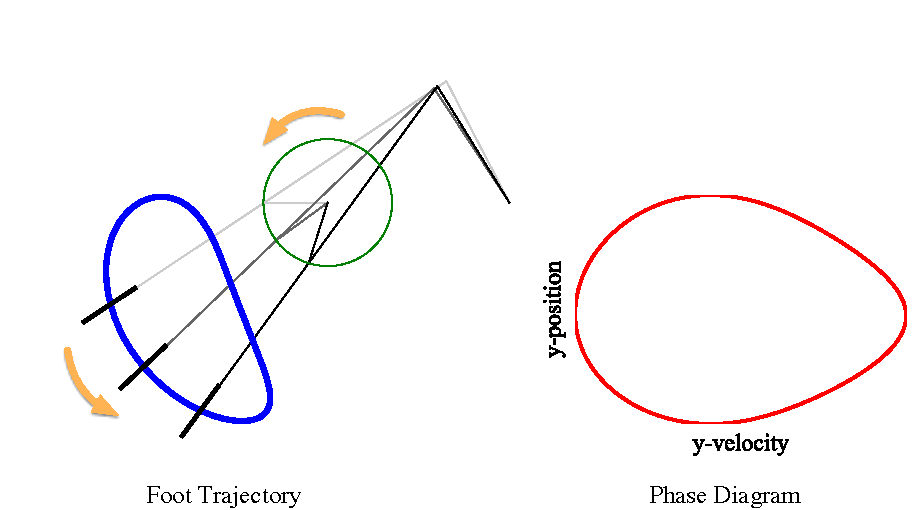
\includegraphics[width = \textwidth]{figures/foot_trajs.pdf}
		\caption{The water runner robot's foot locus in blue, with three instantaneous configurations of the leg's four-bar mechanism shown in grey. The circular path traced by the joint at the end of the input link is traced in green. In red is the phase diagram of this legged system.}
		\label{fig:trajrob}
	\end{subfigure}

	\begin{subfigure}[t]{0.5\textwidth}
		\centering
		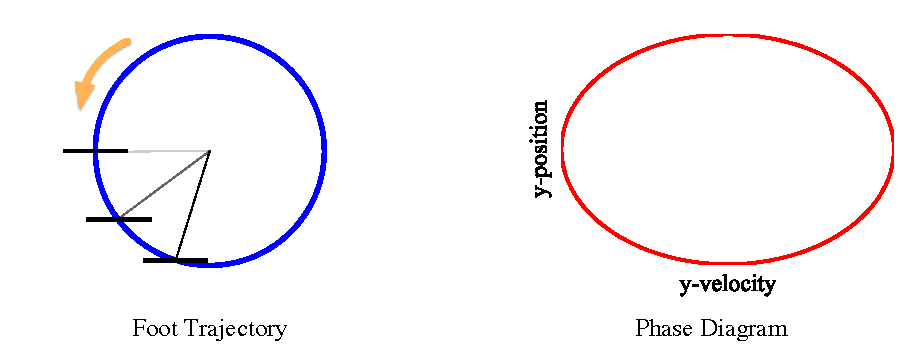
\includegraphics[width = \textwidth]{figures/foot_trajs2.pdf}
		\caption{A simplified circular foot locus in blue, with three instantaneous leg configurations shown in grey. In red is the phase diagram of this model.}
		\label{fig:trajsimp}
	\end{subfigure}
	\caption{Trajectories and phase portraits for the water runner robot and a simplified model. Note that the orientation of the foot pad of the actual robot follows the orientation of the leg, whereas the orientation of the foot pad in the simplified mode is constant.}
	\label{fig:traj}
\end{figure}

Because we are neglecting the horizontal kinematics of the system, the simplified circular foot trajectory can be further simplified to a foot mounted on a prismatic joint traveling vertically. We can calculate the force generated by a foot traveling on this trajectory via the equation obtained by Galsheen and McMahon \cite{glasheen1996vertical}, which states that the time-varying forces exerted by water during vertical impact of disks follows,

\begin{equation}
	F(t) = - C_D^* \left[\frac{1}{2} S \rho \dot{y}(t) |\dot{y}(t) | + S \rho g y(t) \right]
	\label{eq:force_t}
\end{equation}

\noindent where $F(t)$ is the time varying drag force, $C_D^* \approx 0.703$ is the drag coefficient, $\rho$ is the density of water, $g$ is the acceleration due to gravity, $S = \pi r_{eff}^2$ is the effective circular area of the disk, and $y(t)$ and $\dot{y}(t)$ are the time-varying vertical position and velocity of the disk measured in a coordinate system where positive $y$ opposes the gravity vector. 

Equation~\ref{eq:force_t} shows that the magnitude of the force force has a quadratic dependence on foot pad speed, as one would expect given the high-Reynolds number regime in which the foot operates. Therefore, the robot should generate significantly more lift by plunging its foot into the water faster than it retracts its foot.

We now introduce a new parameter, duty factor $(DF)$, which is the ratio of the time the foot spends travelling downwards over the total time of one cycle. With this definition, we can find the angular velocity during the downwards half of the trajectory $\omega_1$ and the angular velocity during the upwards half of the trajectory $\omega_2$, given an average angular velocity $\omega$.

\begin{align}
	\omega_1 &= \frac{\omega}{2 DF} \\
	\omega_2 &= \frac{\omega}{2 (1 - DF)}
\end{align}

\section{CONCLUSIONS}

%\addtolength{\textheight}{-12cm}   % This command serves to balance the column lengths
                                  % on the last page of the document manually. It shortens
                                  % the textheight of the last page by a suitable amount.
                                  % This command does not take effect until the next page
                                  % so it should come on the page before the last. Make
                                  % sure that you do not shorten the textheight too much.

%%%%%%%%%%%%%%%%%%%%%%%%%%%%%%%%%%%%%%%%%%%%%%%%%%%%%%%%%%%%%%%%%%%%%%%%%%%%%%%%

\section*{APPENDIX}

Appendixes should appear before the acknowledgment.

\section*{ACKNOWLEDGMENT}

This material is based upon work supported by the National Science Foundation Graduate Research Fellowship under Grant No. (NSF grant number). Any opinion, findings, and conclusions or recommendations expressed in this material are those of the authors(s) and do not necessarily reflect the views of the National Science Foundation.

\bibliographystyle{IEEEtran}
\bibliography{iros}

\end{document}
